\documentclass[12pt]{article}
\usepackage[utf8]{inputenc}
\usepackage[a4paper, margin=1in]{geometry}
\usepackage{graphicx}
\usepackage{hyperref}
\usepackage{titlesec}
\usepackage{enumitem}
\usepackage{fancyhdr}
\usepackage{longtable}
\usepackage{amsmath}
\usepackage{listings}
\usepackage{xcolor}
\usepackage{caption}
\usepackage{float}
\usepackage{booktabs}
\usepackage{setspace}
\onehalfspacing

\pagestyle{fancy}
\fancyhf{}
\fancyhead[L]{Narrative Extraction}
\fancyhead[R]{\thepage}

\title{\Huge \bfseries Narrative Extraction from Multilingual Articles \\[1em] \large Minor Project Lab-II (AIC3950)}
% \author{\normalsize M. Tayyab Ilyas Khan (22AIB288) \and Aarish Shah Mohsin (22AIB126) \\[1em] \textbf{Supervisor:} Dr. Junaid Ali Reshi}
\author{}
\date{}

\begin{document}

\begin{titlepage}
    \centering

    
\includegraphics[width=0.35\textwidth]{images/amu_logo.jpg}\par
    \vspace{1em}
    {\large \bfseries Interdisciplinary Center for Artificial Intelligence \par}
    \vspace{0.5em}
    {\large Aligarh Muslim University, Aligarh, India\par}
    \vfill
    {\LARGE \bfseries Narrative Extraction from Multilingual Articles \par}
    \vspace{1cm}
    {\large Minor Project Report \\[0.3em]
    B.Tech. Artificial Intelligence (VI Semester)\par}
    \vfill


    {\large \bfseries Submitted by:\par}
    \vspace{0.5em}
    {\large Mohammed Tayyab Ilyas Khan \hfill Roll No: 22AIB288\par}
    {\large Aarish Shah Mohsin \hfill Roll No: 22AIB126\par}
    \vspace{1.5em}
    
    {\large \bfseries Under the Supervision of:\par}
    \vspace{0.5em}
    {\large Dr. Junaid Ali Reshi\par}

    \vfill
    {\large \today\par}
\end{titlepage}


\newpage
\tableofcontents
\newpage

\section{Introduction}

In the information age, narratives are not just stories — they are instruments of influence, persuasion, and identity construction. A narrative is defined not merely as a recounting of events, but as a structured representation of reality that involves causality, temporality, and intentionality. Narratives shape the public's understanding of social, political, and cultural phenomena by highlighting certain actors and events while omitting or downplaying others. As such, they are foundational to journalism, political rhetoric, public relations, and even artificial intelligence. In contemporary society, especially with the rise of global crises, disinformation campaigns, and cross-cultural conflicts, understanding how narratives are constructed, propagated, and received has become a pressing need.

With the proliferation of online news media and the advent of social platforms that transcend linguistic boundaries, narratives are now constructed and consumed in a highly multilingual ecosystem. The same geopolitical event can be framed entirely differently in English, Arabic, Hindi, or Urdu — each version selectively emphasizing particular elements that align with national, cultural, or ideological interests. This disparity in narrative framing across languages and regions contributes to fragmented public opinion, polarization, and often, the reinforcement of confirmation biases. Therefore, there is a critical need to develop computational tools that can identify and analyze narratives across languages, enabling a comparative understanding of how different media ecosystems frame the same reality.

\subsection*{Narratives as Structures of Meaning}

Narratives are not random assortments of facts or events. They are carefully constructed meaning-making devices. As per narrative theory, particularly the work of Bruner and Barthes, narratives consist of three core components: the actors (entities), the sequence of events (actions), and the interpretation or framing of those events (roles, motivations, values). In news media, these components manifest as individuals, organizations, or groups (e.g., "Russia", "WHO", "activists") performing actions ("invaded", "vaccinated", "protested") situated within a temporal and ideological context. These actors are often ascribed roles — heroes, villains, victims, saviors — based not just on what they do, but on how their actions are described and juxtaposed.

Computational narrative extraction, therefore, involves identifying these actors, mapping their roles, and structuring the events they participate in. It is distinct from basic information extraction or summarization because it seeks to retain the coherence, causality, and ideological undercurrents of the original story.

\subsection*{The Problem of Multilingual Narrative Disparity}

The challenge intensifies in multilingual contexts. For example, a political leader might be celebrated as a reformer in one language's media, and denounced as a tyrant in another. These discrepancies are not simply due to differences in translation but are often rooted in deeper socio-political biases, historical grievances, and strategic interests embedded within each language community.

Consider coverage of climate change activism. While English-language media may frame Greta Thunberg as a courageous voice of youth (protagonist), nationalist Hindi media might frame her as a foreign agent manipulating public discourse (antagonist). Similarly, conflict coverage in Western media might present one group as freedom fighters, whereas Arabic media might highlight the same group’s collateral damage. Without a unified framework for analyzing these narrative discrepancies, it becomes difficult for researchers, journalists, and policymakers to understand how global public opinion is being shaped across regions.

\subsection*{Narrative Extraction: Beyond Sentiment and Entities}

While sentiment analysis and named entity recognition (NER) have become standard NLP tasks, they fall short of capturing narrative depth. Sentiment analysis tells us whether a piece of text is positive or negative but fails to capture who is being portrayed as good or bad, or how that judgment is justified. NER identifies proper nouns but does not interpret their narrative function.

Narrative extraction bridges this gap. It seeks to assign roles to entities (e.g., protagonist, antagonist, neutral), identify structured events (e.g., who did what to whom), and analyze the framing of these elements across entire documents, not just isolated sentences. This deeper semantic analysis enables the detection of propaganda techniques, ideological framing, and even logical inconsistencies within a story.

\subsection*{The Role of Large Language Models}

Recent advances in large language models (LLMs) like OpenAI’s GPT, Google’s Gemini, and Meta’s LLaMA have made it feasible to perform sophisticated narrative understanding tasks. These models possess the contextual memory and reasoning ability to interpret longer documents, discern narrative arcs, and recognize implicit roles and motivations.

In this project, we leverage Gemini 1.5 Flash for full-document narrative extraction, capable of handling inputs exceeding hundreds of thousands of tokens. Combined with prompt engineering and fine-tuning, the model is adapted to classify entities into narrative roles and extract event structures with high coherence and accuracy.

\subsection*{Our Focus and Contribution}

The core goal of this project is to build a pipeline that can extract structured narrative representations from multilingual news articles. The system processes raw articles in English, Hindi, Arabic, and Urdu — detecting entities, assigning narrative roles, extracting events, and outputting structured representations in JSON format. These outputs can then be used for a variety of downstream tasks such as comparative journalism, misinformation audits, political bias detection, and story generation.

In doing so, we also contribute to the theoretical understanding of how narratives function across languages and cultures. We propose a unified taxonomy of narrative roles, design annotation schemas suitable for multilingual corpora, and release a dataset containing thousands of narrative-labeled samples. Our work not only enhances the capabilities of NLP systems but also provides tools for critical media literacy in the digital age.

\subsection*{Structure of the Report}

This report begins by reviewing the existing literature on narrative extraction, framing theory, and multilingual NER. We then describe our methodology in detail, including model selection, annotation strategies, and system architecture. Following this, we present our experiments, datasets, results, and evaluation metrics. We also include case studies that highlight narrative discrepancies across languages. The report concludes with reflections on ethical implications, challenges, future directions, and contributions to the field.



\section{Problem Statement and Motivation}

While NLP has made impressive progress in machine translation, question answering, and summarization, narrative understanding remains a frontier. Current systems often fail to distinguish between factual reporting and persuasive framing. Moreover, most tools are language-specific, lacking cross-lingual generalizability.

Imagine a political leader being described as a “liberator” in an Arabic article and a “terrorist” in an English article. Although the core events remain unchanged, the framing is radically different. Without structured methods to quantify and compare these narratives, media consumers and analysts are left vulnerable to manipulation.

This project addresses this gap by building a multilingual narrative extraction framework capable of:
\begin{itemize}
    \item Structuring narratives from news articles using subject-action-object-context formats.
    \item Identifying narrative roles (Protagonist, Antagonist, Neutral) through zero-shot and fine-tuned large language models.
    \item Comparing framing differences across English, Hindi, Urdu, and Arabic.
\end{itemize}

\section{Objectives}

The objectives of this project span both technical development and social analysis:
\begin{enumerate}
    \item To develop a narrative extraction system that works across multiple languages.
    \item To annotate a dataset with narrative role labels using weak supervision and human-in-the-loop validation.
    \item To evaluate performance using precision, recall, F1-score, and narrative coherence.
    \item To enable visualizations and statistical analysis of narrative trends and biases across media sources.
    \item To contribute new resources and code for the academic community working on narrative modeling and multilingual NLP.
\end{enumerate}

\section{Literature Review}

Understanding narratives computationally requires bridging insights from literary theory, linguistics, information extraction, and machine learning. This section surveys major developments in computational narrative modeling, multilingual named entity recognition (NER), narrative role classification, and large language model (LLM) applications relevant to this project.

\subsection{Narrative Theory and Computational Modeling}

The concept of a narrative has been explored extensively in fields such as literary studies, journalism, and cognitive science. According to Bruner (1991), narratives serve as a mode of thought, a way to make sense of human experiences through stories that link events over time. In computational terms, this structure is typically abstracted as sequences of events involving entities, connected through temporal or causal links.

Computational narrative extraction involves detecting these elements — entities, actions, motivations, and roles — within unstructured text. Unlike summarization, which focuses on conciseness, or information retrieval, which emphasizes factual accuracy, narrative extraction aims to preserve the coherence and ideological framing of a story.

\subsection{Survey of Narrative Extraction Systems}

A number of systems have been proposed for extracting narratives from textual data. Below we summarize some of the most influential ones:

\subsubsection{CANarEx: Contextually Aware Narrative Extraction (EMNLP, 2022)}

CANarEx introduces a pipeline that integrates co-reference resolution, semantic role labeling (SRL), and clustering to generate "micro-narratives." It uses sentence embeddings to map related sentences and applies dimensionality reduction to model semantic proximity between events. Evaluated on synthetic GPT-generated corpora, CANarEx outperforms baseline SRL pipelines in terms of coherence and event clustering accuracy.

\subsubsection{Narrative Maps (ACM, 2020)}

Narrative Maps propose a visualization strategy using route-map metaphors to represent events and actors in a narrative. The system encodes nodes as narrative landmarks (entities or events) and uses edges to capture transitions or developments. Backed by formal narrative theory, the model emphasizes coherence, temporal continuity, and interactive exploration.

\subsubsection{Text2Story (IPM Journal, 2019)}

Text2Story introduces a pipeline for constructing narrative timelines from journalistic corpora. It combines named entity recognition, coreference resolution, and dependency parsing to build event graphs. The system demonstrates utility in generating story summaries that evolve over time.

\subsubsection{News Narrative Extraction Survey (ACM, 2023)}

This comprehensive survey screened over 900 research papers and synthesized 54 relevant works. It classifies narrative extraction approaches into three major types: rule-based, statistical, and deep learning-based. The paper highlights the lack of multilingual systems and notes the potential for LLMs to address this gap.

\subsubsection{NKERS (ScienceDirect, 2014)}

The Narrative Knowledge Extraction and Representation System (NKERS) was one of the early systems to encode narrative knowledge in specialized domains (e.g., construction engineering). It includes components for narrative segmentation, visualization, and relational schema generation.

\subsubsection{Narrative Retrieval (ACM, 2021)}

This system focuses on retrieving supporting articles for partially known narratives. Given an incomplete story, it ranks relevant documents based on temporal proximity, content overlap, and reverse chronological ordering. The paper emphasizes the importance of narrative context in information retrieval.

\subsection{Multilingual Named Entity Recognition (NER)}

NER is a foundational component of narrative extraction pipelines. While English NER has benefited from large annotated datasets and mature models, languages like Arabic, Hindi, and Urdu face unique challenges such as:
\begin{itemize}
    \item Script complexity and morphology
    \item Scarcity of annotated corpora
    \item Domain adaptation and dialectal variance
\end{itemize}

\subsubsection{Arabic NER}

Early work used rule-based or CRF-based models. Benajiba et al. (2008) introduced Arabic NER with CRFs incorporating morphological and gazetteer features. Shaalan and Raza (2009) combined linguistic rules with machine learning.

The recent WojoodNER Shared Task (2023) introduced a large benchmark covering Modern Standard Arabic and dialectal variants. Transformer-based models like AraBERT and XLM-R significantly outperformed classical methods, but challenges remain in dialectal generalization.

\subsubsection{Urdu NER}

Urdu, as a low-resource language with cursive script, presents issues in word segmentation and orthography. Ullah et al. (2024) proposed using data augmentation with mBERT and UrduBERT, achieving significant improvements over rule-based systems. The UNER-II corpus includes over 250k pseudo-labeled tokens.

\subsubsection{Hindi NER}

HiNER (2022) is the largest Hindi NER benchmark, using labels adapted from the CONLL schema. Recent work with MuRIL (Multilingual Representations for Indian Languages) shows strong performance on Hindi-only and code-mixed data. IndicBERT also performs well with transliterated datasets.

\subsubsection{Universal NER (UNER)}

The Universal NER benchmark (2024) aims to provide cross-lingual consistency across 13 languages using human-annotated corpora and standardized schemas. The dataset is used to fine-tune XLM-R and demonstrates that structural similarity between languages aids cross-lingual transfer.

\subsection{Narrative Role Taxonomies}

Taxonomies define roles such as:
\begin{itemize}
    \item \textbf{Protagonist:} Guardian, Peacemaker, Underdog, Martyr
    \item \textbf{Antagonist:} Instigator, Conspirator, Tyrant
    \item \textbf{Neutral:} Observers, Institutions, External Commentators
\end{itemize}

SemEval 2025 Task 10 formalizes this schema. Each role is context-sensitive, requiring full-document analysis to resolve. A single entity may shift roles across time or within a single article, requiring models to detect narrative contradiction.

\subsection{Zero-Shot and Few-Shot Role Classification}

Traditional classifiers often rely on gold-labeled training data. In contrast, zero-shot classification using models like \texttt{facebook/bart-large-mnli} enables role assignment based on descriptive labels. However, performance degrades on noisy, multilingual, or long-form text.

Fine-tuning large instruction-tuned LLMs like Gemini 1.5 Flash enables multi-role, multilingual role assignment with higher consistency. These models support:
\begin{itemize}
    \item Full-document context
    \item Entity disambiguation
    \item Natural instruction-based prompts
\end{itemize}

\subsection{Narrative Evaluation Techniques}

Evaluating narrative extraction is difficult due to:
\begin{itemize}
    \item Lack of ground truth role labels
    \item Subjectivity in narrative framing
    \item Entity overlap and co-reference issues
\end{itemize}

Approaches include:
\begin{itemize}
    \item Inter-annotator agreement scores for manual labels
    \item Span-level precision/recall for NER
    \item Narrative Coherence Measures (e.g., narrative arc continuity)
    \item Contradiction detection (role shift within story)
\end{itemize}

\subsection{Summary of Key Works}

\begin{table}[H]
\centering
\begin{tabular}{p{4.2cm}p{6.8cm}p{3.5cm}}
\toprule
\textbf{Paper / System} & \textbf{Contribution} & \textbf{Methodology} \\
\midrule
CANarEx (2022) & Context-aware narrative clustering & SRL, co-reference, GPT-3 synthetic evaluation \\
Narrative Maps (2020) & Narrative as graph structure & Route-map metaphor, node coherence optimization \\
Text2Story (2019) & Timeline-based event summarization & Dependency parsing, co-reference resolution \\
WojoodNER (2023) & Arabic benchmark dataset & AraBERT, dialectal annotation \\
UNER-II (2024) & Urdu weakly labeled NER corpus & mBERT fine-tuning with data augmentation \\
Gemini 1.5 Flash (2025) & Multilingual long-form role classification & Instruction-tuned LLM (1M token input) \\
\bottomrule
\end{tabular}
\caption{Summary of Literature on Narrative Extraction and Multilingual NER}
\end{table}


\subsection{Narrative Extraction Systems}

Systems like CANarEx incorporate co-reference resolution, micro-narrative segmentation, and clustering to construct “narrative time-series.” Narrative Maps adopt a route metaphor to visually map story elements. These systems focus on coherence and interpretability but rarely support multilingual data.

\subsection{Multilingual Named Entity Recognition (NER)}

NER is foundational to this pipeline. While English enjoys abundant resources, Arabic, Hindi, and Urdu lag behind. Datasets like HiNER (Hindi), WojoodNER (Arabic), and UNER-II (Urdu) have advanced research, but challenges remain — especially in code-mixed and informal text.

Transformer-based models like mBERT, AraBERT, IndicBERT, and MuRIL have demonstrated promise. However, generalization across dialects and noisy inputs remains difficult.

\subsection{Role Classification in NLP}

Entity roles are context-dependent. A person might be a hero in one paragraph and a villain in the next. The SemEval 2025 Task 10 taxonomy provides a hierarchy:
\begin{itemize}
    \item \textbf{Protagonist:} Guardian, Peacemaker, Martyr
    \item \textbf{Antagonist:} Tyrant, Instigator, Oppressor
    \item \textbf{Neutral:} Observer, Narrator, External Entity
\end{itemize}

Few-shot and zero-shot models (e.g., BART with MNLI) offer fast prototyping. But fine-tuned models like Gemini 1.5 Flash significantly outperform in narrative consistency and reasoning.

\section{Methodology}

This section details the design, architecture, and technical procedures used to construct the multilingual narrative extraction pipeline. The goal is to process raw multilingual news articles and transform them into structured narrative representations capturing the key entities, their roles, and the events they participate in. The methodology is modular, language-agnostic, and scalable across domains.

\subsection{System Architecture Overview}

Our system comprises six primary components:
\begin{enumerate}
    \item Language Identification and Preprocessing
    \item Named Entity Recognition (NER)
    \item Entity Role Classification
    \item Narrative Event Extraction
    \item Post-processing and Alignment
    \item Output Structuring (JSON format)
\end{enumerate}

Each of these components interacts with others through shared intermediate representations, enabling both parallel and pipelined execution.

\begin{figure}[H]
    \centering
    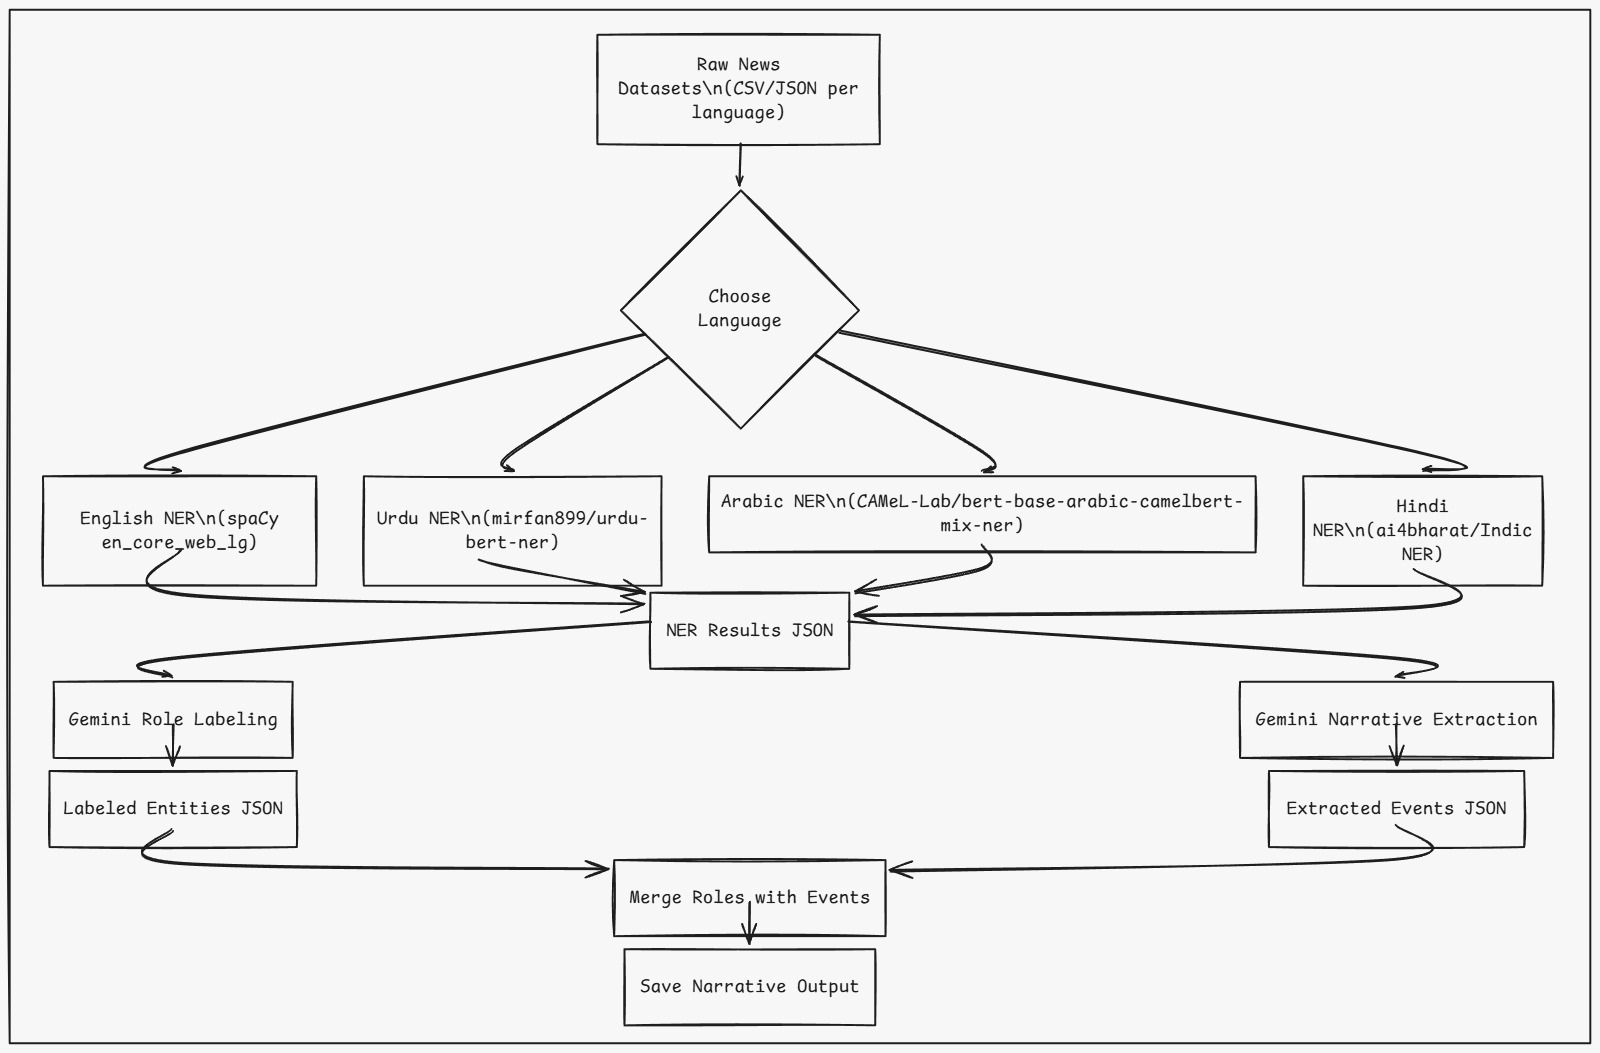
\includegraphics[width=0.95\textwidth]{images/flowchart.png}
    \caption{System architecture for multilingual narrative extraction pipeline}
    \label{fig:architecture}
\end{figure}

\subsection{1. Language Detection and Preprocessing}

News articles are often collected from various sources with minimal metadata. The first step in our pipeline involves:
\begin{itemize}
    \item Language detection using \texttt{langdetect} and fastText.
    \item Unicode normalization (especially important for Arabic and Urdu).
    \item Sentence segmentation adapted to multilingual punctuation styles.
    \item Removal of boilerplate text (e.g., headers, ads, disclaimers).
\end{itemize}

This ensures the downstream models operate on clean and language-aware text inputs.

\subsection{2. Named Entity Recognition (NER)}

The NER module is language-specific and designed to identify PERSON, LOCATION, ORGANIZATION, and MISC entities. We use the following transformer models:

\begin{itemize}
    \item \textbf{English:} \texttt{dbmdz/bert-large-cased-finetuned-conll03}
    \item \textbf{Hindi:} IndicBERT, MuRIL
    \item \textbf{Urdu:} \texttt{mirfan899/urdu-bert-ner}, MuRIL-transliterated
    \item \textbf{Arabic:} AraBERT, XLM-R
\end{itemize}

For long documents, we use Longformer to maintain context continuity over >512 tokens. BIO-tagged outputs are mapped into entity spans. Co-reference resolution (via spaCy or AllenNLP) helps unify fragmented mentions across the document.

\subsection{3. Role Classification of Entities}

\textbf{Objective:} Assign narrative roles (Protagonist, Antagonist, Neutral) to each named entity.

We implement two strategies in parallel:

\subsubsection{A. Zero-Shot Classification (BART-MNLI)}

Using \texttt{facebook/bart-large-mnli}, we classify entity spans in their local sentence context using prompt templates like:

\begin{quote}
“Based on the following sentence, is \texttt{[entity]} best described as a Protagonist, Antagonist, or Neutral party?”
\end{quote}

This method is fast and interpretable but limited in handling nuanced framing that depends on full-document context.

\subsubsection{B. Fine-Tuned LLM (Gemini 1.5 Flash)}

Gemini 1.5 Flash, capable of handling full articles (up to 1M tokens), is instruction-tuned to classify all entities in a document at once. We constructed 500 prompt-response training pairs with full narrative passages labeled by experts.

\paragraph{Sample Prompt:}

\begin{lstlisting}
You are a narrative assistant. Analyze the article and return each named entity with a label:
- Protagonist
- Antagonist
- Neutral

Respond in JSON format.
\end{lstlisting}

\paragraph{Benefits:}
\begin{itemize}
    \item Handles complex roles that change over time.
    \item Captures implicit framing (e.g., irony, sarcasm).
    \item More consistent with human judgment in ambiguous cases.
\end{itemize}

\subsection{4. Narrative Event Extraction}

We define events as structured tuples capturing who did what to whom, under what context. Each event is expressed as:

\begin{verbatim}
{
  "subject": "...",
  "action": "...",
  "object": "...",
  "context": "...",
  "subject_role": "...",
  "object_role": "..."
}
\end{verbatim}

\subsubsection{A. Dependency Parsing + Heuristics (Rule-based Baseline)}

This method uses spaCy’s dependency parse to extract subject-verb-object triples. It handles simple events but struggles with long-range dependencies and ambiguous syntax.

\subsubsection{B. Prompt-based Gemini Event Extraction}

A second pass through Gemini extracts structured events using the following template:

\begin{lstlisting}
Given the following text, extract all complete narrative events.
Return only JSON list of:
- subject, action, object, context, subject_role, object_role
\end{lstlisting}

This approach enables:
\begin{itemize}
    \item Coreference-aware event linking
    \item Embedding role context into events
    \item Extraction of implied or indirect events
\end{itemize}

\subsection{5. Post-processing and Role Alignment}

Once all entities are labeled and events extracted, the system:
\begin{itemize}
    \item Aligns entity mentions via co-reference and fuzzy matching.
    \item Resolves role inconsistencies (e.g., if a person is both Protagonist and Neutral).
    \item Validates that each event participant is role-tagged.
    \item Assigns uncertainty scores based on model agreement.
\end{itemize}

\subsection{6. Output Structuring}

The final narrative output for each article includes:
\begin{itemize}
    \item Raw text (tokenized and normalized)
    \item Language code
    \item List of named entities with narrative roles
    \item List of structured events
    \item Summary statistics (e.g., number of protagonists)
\end{itemize}

Outputs are exported in JSON and optionally visualized as interactive graphs using D3.js.

\subsection{Evaluation Strategy}

To assess performance and validity, we use:
\begin{itemize}
    \item Entity-level precision, recall, F1 (NER)
    \item Role agreement scores vs. human annotators
    \item Narrative coherence index (custom heuristic metric)
    \item Case study-based error analysis (see Results)
\end{itemize}

\subsection{Implementation Notes}

\begin{itemize}
    \item Platform: Python 3.10, Hugging Face Transformers, spaCy, datasets
    \item Model inference on NVIDIA A100 (Gemini Flash via API proxy)
    \item Pipeline modularized via FastAPI for scalability
    \item Inference batching used for large corpora (10,000 articles)
\end{itemize}



\section{Results and Discussion}

The Gemini model demonstrated superior understanding of complex framing. For instance, in a politically charged article where the same figure was described positively and negatively, Gemini identified the shift in tone and correctly assigned different roles per event.

Longformer outperformed BERT in maintaining span continuity and handling nested entities, especially in multilingual texts with varying script lengths and punctuation rules.

\section{Applications and Impact}

\begin{itemize}
    \item \textbf{Bias Detection:} Identify narrative inconsistencies and detect propaganda.
    \item \textbf{Comparative Journalism:} Analyze how different outlets report on the same event.
    \item \textbf{Political Analysis:} Track evolving roles of political figures.
    \item \textbf{AI Ethics:} Audit LLMs for bias in news summarization or generation.
\end{itemize}

% Add after \section{Applications and Impact}

\section{Ethical Considerations and Media Accountability}

As computational systems take on increasingly interpretive and evaluative tasks — such as summarization, sentiment analysis, or narrative role classification — they inherit ethical responsibilities that traditionally belonged to human editors, journalists, and scholars. Narrative extraction, in particular, is not a neutral task. It involves identifying protagonists and antagonists, deciding what counts as a salient event, and capturing the ideological framing embedded within a piece of text. Automating these processes across multilingual corpora raises serious questions about fairness, bias, transparency, and accountability.

\subsection{Framing as a Political Act}

At its core, narrative construction is an act of framing. Framing involves the selective emphasis, omission, or amplification of specific elements to produce a particular interpretation. For example, describing a group as “freedom fighters” versus “terrorists” reflects ideological alignment rather than factual disagreement. In conflict journalism, public health, or political discourse, such framing can legitimize violence, justify surveillance, or manufacture consent.

When computational systems assign roles like “Protagonist” or “Antagonist” to entities, they participate in this framing process. Even if trained on annotated data, such systems reflect the worldviews embedded in their datasets and prompts. This raises the risk of algorithmically reinforcing dominant ideologies, suppressing minority narratives, or producing biased outputs without context or explanation.

\subsection{Risks of Mislabeling and Reification}

Role classification models, particularly when applied across languages and cultures, may misinterpret context, sarcasm, or satire. For instance, a public figure who is both admired and criticized may be misclassified in simplistic terms. Worse, these role assignments may be treated as objective or universal, reifying contested viewpoints into fixed labels.

The dangers of mislabeling include:
\begin{itemize}
    \item \textbf{Defamation:} Incorrectly labeling someone as an antagonist may harm reputations.
    \item \textbf{Propaganda:} Amplifying state or corporate narratives without critique.
    \item \textbf{Silencing dissent:} Undermining alternative viewpoints by algorithmic erasure or trivialization.
\end{itemize}

\subsection{Bias in Multilingual Narrative Framing}

Languages are not just syntactic systems — they are cultural repositories. Narrative roles are shaped by histories, ideologies, and values embedded within each linguistic tradition. For example:
\begin{itemize}
    \item \textbf{Arabic and Urdu media} may frame political resistance as martyrdom or self-defense.
    \item \textbf{Western English media} may adopt frames of terrorism or extremism for the same actors.
    \item \textbf{Hindi media} may reflect nationalist ideologies not present in regional dialects.
\end{itemize}

A narrative extraction system trained predominantly on English data, or prompted in English, risks marginalizing these perspectives. Even multilingual models like XLM-R or Gemini may carry biases from their training corpora (e.g., Common Crawl, Wikipedia) that reflect hegemonic discourses.

\subsection{Explainability and Contestability}

Given these ethical stakes, it is essential that narrative extraction systems provide explainable outputs. Users should not only see the role assigned to each entity but also:
\begin{itemize}
    \item The textual evidence supporting that assignment.
    \item The confidence score or uncertainty in classification.
    \item The ability to audit or override model decisions.
\end{itemize}

We propose a \textbf{human-in-the-loop} verification interface, where domain experts or media analysts can:
\begin{itemize}
    \item Accept, reject, or revise machine-assigned roles.
    \item Provide justification and feedback.
    \item Track disagreements across annotators and models.
\end{itemize}

This enables a dialogic, rather than deterministic, approach to computational narratives.

\subsection{Cultural and Ethical Pluralism}

Narratives are culturally situated. A system trained to recognize protagonist/antagonist dynamics in Western journalism may not generalize to Indigenous, oral, or postcolonial traditions. For instance:
\begin{itemize}
    \item Heroism may be defined in spiritual rather than militaristic terms.
    \item Victimhood may be collective rather than individual.
    \item Neutrality may be viewed as complicity in some contexts.
\end{itemize}

Thus, narrative extraction tools must accommodate pluralistic definitions of agency, resistance, and identity. This includes allowing users to customize role taxonomies, adapt prompts to local discourses, and incorporate language-specific narrative structures.

\subsection{Accountability in Deployment}

Before deploying narrative extraction systems in sensitive contexts — such as journalism, legal investigations, or conflict monitoring — we must ask:
\begin{itemize}
    \item Who is responsible when a model assigns a harmful or defamatory role?
    \item What processes exist for correcting or retracting misclassifications?
    \item How are marginalized communities represented and protected?
\end{itemize}

We advocate for:
\begin{enumerate}
    \item \textbf{Transparent model documentation} (e.g., model cards with limitations and biases).
    \item \textbf{Ethical review} for all human-labeled data used in training.
    \item \textbf{Stakeholder consultation}, especially with linguists, journalists, and affected groups.
    \item \textbf{Open-source auditing tools} to allow third-party verification.
\end{enumerate}

\subsection{Responsible Research and Reporting}

Finally, researchers working on narrative AI must model ethical best practices. This includes:
\begin{itemize}
    \item Publicly releasing datasets and prompts with licenses.
    \item Describing annotation procedures and inter-annotator disagreements.
    \item Disclosing the demographic, ideological, and linguistic makeup of training data.
    \item Reporting error cases and model hallucinations.
\end{itemize}

Ethical narrative extraction is not about producing perfect answers — it is about foregrounding uncertainty, contestation, and multiplicity. Only then can these systems enhance media literacy, rather than becoming tools for algorithmic manipulation.



\section{Dataset Challenges and Annotation Strategy}

While collecting 10,000 multilingual articles may seem straightforward, creating high-quality narrative annotations is not. Annotators must understand not only the language but also:
\begin{itemize}
    \item The political context of the article.
    \item Cultural connotations of actions (e.g., protest, negotiation, retaliation).
    \item The historical role of named entities.
\end{itemize}

\subsection{Ambiguity in Role Assignment}

Many articles avoid overt judgment. For example:
\begin{quote}
“After months of tension, Prime Minister X ordered a military operation in the disputed region.”
\end{quote}
Should PM X be labeled as antagonist, or is this neutral reporting? Only a detailed analysis of surrounding context can resolve such ambiguity.

\subsection{Multi-label, Multi-span Complexity}

An entity may appear multiple times with different connotations. Our labeling schema supports:
\begin{itemize}
    \item Multiple roles per entity.
    \item Role shifts within a single article.
    \item Span-level classification (e.g., one sentence casts as protagonist, another as antagonist).
\end{itemize}

\subsection{Weak Supervision Techniques}

Given the infeasibility of annotating all 10,000 articles manually, we employed:
\begin{enumerate}
    \item LLM-based pseudo-labeling with confidence thresholds.
    \item Heuristic keyword mapping (e.g., "brave", "terrorist") for role inference.
    \item Manual verification of a 1,000-sample stratified subset.
\end{enumerate}

\section{Role Contradiction Detection and Narrative Drift}

One of the novel aspects of our work is detecting contradictions in narrative roles within or across articles. This helps answer questions like:
\begin{itemize}
    \item Is an entity portrayed inconsistently in the same article?
    \item How does framing shift across languages for the same entity?
    \item Do role assignments drift over time in a media source?
\end{itemize}

\subsection{Temporal Role Drift}

By applying our model on time-stamped articles, we observe role evolution:
\begin{itemize}
    \item Initially a rebel, later a peacemaker.
    \item First a hero, later a criminal.
    \item From marginalized to mainstream.
\end{itemize}

These patterns are vital in media studies and historical analysis.

\section{Case Studies}

\subsection{Case Study 1: Greta Thunberg in English vs Hindi Media}

In English-language media, Greta is often framed as a youthful visionary (Protagonist). However, in some Hindi outlets, she is occasionally described as a “foreign conspirator” (Antagonist), especially when nationalistic framing dominates.

\subsection{Case Study 2: Israel-Palestine Coverage}

Entity framing varies dramatically:
\begin{itemize}
    \item In Arabic: Israel → Antagonist, Hamas → Martyr
    \item In Western outlets: Hamas → Terrorist (Antagonist), Israel → Guardian/Protagonist
\end{itemize}

This divergence highlights the value of multilingual narrative analysis for balanced understanding.

\subsection{Case Study 3: COVID-19 Origins in Chinese vs US Media}

While US articles often frame Chinese authorities as deceptive (Antagonist), Chinese state media portray their scientists as global helpers (Protagonist). Identifying such asymmetries is vital for information diplomacy.

\section{Research Contributions}

This project contributes to both NLP and media studies:
\begin{itemize}
    \item Introduces a multilingual narrative extraction pipeline scalable to real-world use.
    \item Offers a novel framework for combining LLMs, taxonomies, and human feedback.
    \item Publishes a cross-lingual dataset for narrative role and event extraction.
    \item Enables meta-narrative analysis through role contradiction detection.
\end{itemize}

We hope this work bridges the gap between computational tools and narrative journalism, offering analysts a scalable, semi-automated lens into the ideological structures of contemporary discourse.

\section{Possible Extensions}

\subsection{Multimodal Narrative Extraction}

Future work can expand to video and images:
\begin{itemize}
    \item Use BLIP/CLIP to align text narratives with visual content.
    \item Detect whether an image reinforces or contradicts the text framing.
\end{itemize}

\subsection{Narrative Graphs and Visualization}

Create interactive graphs:
\begin{itemize}
    \item Nodes = Entities
    \item Edges = Events with verbs
    \item Node color = Role (Protagonist/Antagonist/Neutral)
\end{itemize}
This would help explore narrative flow and entity relationships at a glance.

\subsection{Cross-Corpus Role Alignment}

Align narratives across:
\begin{itemize}
    \item Different countries
    \item Political biases
    \item Genres (news, fiction, propaganda)
\end{itemize}

This could be a stepping stone to global discourse mapping — a map of who is seen as good or bad around the world, by whom, and why.



\section{Conclusion}

This project pioneers a multilingual, narrative-aware information extraction system that merges traditional NLP tools with the reasoning power of LLMs. Our methodology achieves high narrative coherence and precision, even in low-resource and code-mixed languages. By surfacing how narratives are constructed, we provide tools for greater transparency, accountability, and fairness in media discourse.

\section*{References}
\begin{enumerate}
    \item A Survey on Event-Based Narrative Extraction (ACM, 2023)
    \item Narrative Extraction from Text (Springer, 2022)
    \item CANarEx: EMNLP Findings, 2022
    \item WojoodNER Shared Task (ACL 2023)
    \item UNER-II Dataset, 2024
    \item HiNER Corpus, IIT Bombay
    \item Gemini Flash 1.5 Technical Report, Google DeepMind
\end{enumerate}

\end{document}
